\documentclass[a4paper, 10pt]{article}
\usepackage[utf8]{inputenc} % Change according your file encoding
\usepackage{graphicx}
\usepackage{url}
\usepackage{listings}
\usepackage{xcolor}
\usepackage{caption}
\usepackage{multirow}
\usepackage{pgfplots}
\graphicspath{ {./images/} }

%opening
\title{Seminar Report: Optyyyyy}
\author{\textbf{Juan Pablo Royo Sales, Alicia Vila Rodriguez and} \\\and \textbf{Sergi Palomas Martinez}}
\date{\normalsize\today{}}

\begin{document}

\maketitle

\section{Performance}

\subsection{Experiments}

\begin{itemize}
  \item $(i)$ Different number of clients

  \begin{table}[h!]
  \begin{tabular}{ |c|c|c|c| }
    \hline
    \multicolumn{4}{|c|}{Concurrent Clients - Duration 3s} \\
    \hline
    Experiment & Total Transactions & OK Transactions & \% Transactions\\
    \hline
    \multirow{4}{3cm}{3 CLIENTS \\ 5 ENTRIES \\ 1 RDxTR \\ 1 WRxTR}
    & 95846 & 91049 &  94.99509630031508 \%\\
    & 95921 & 91253 &  95.13349527215104 \%\\
    & 95735 & 91007 &  95.06136731602862 \%\\
    & & &\\
    \hline
    \multirow{8}{3cm}{8 CLIENTS \\ 5 ENTRIES \\ 1 RDxTR \\ 1 WRxTR}
    & 40681 & 34438 &  84.65376957301935 \%\\
    & 40468 & 34183 &  84.46921024018978 \%\\
    & 40652 & 34386 &  84.5862442192266 \%\\
    & 40685 & 34367 &  84.47093523411577 \%\\
    & 40562 & 34355 &  84.69750012326809 \%\\
    & 40761 & 34513 &  84.6716223841417 \%\\
    & 40566 & 34346 &  84.66696248089534 \%\\
    & 40694 & 34421 &  84.58495109844203 \%\\
    \hline

    \multirow{13}{3cm}{13 CLIENTS \\ 5 ENTRIES \\ 1 RDxTR \\ 1 WRxTR}
    & 26690 & 20729 &  77.66579243162234 \%\\
    & 26656 & 20670 &  77.54351740696279 \%\\
    & 26706 & 20640 &  77.2860031453606 \%\\
    & 26709 & 20742 &  77.65921599460856 \%\\
    & 26708 & 20904 &  78.2686835405122 \%\\
    & 26706 & 20867 &  78.13599940088369 \%\\
    & 26700 & 20695 &  77.50936329588015 \%\\
    & 26793 & 20880 &  77.93080282163251 \%\\
    & 26782 & 20736 &  77.42513628556493 \%\\
    & 26794 & 20845 &  77.79726804508472 \%\\
    & 26742 & 20691 &  77.37267220103209 \%\\
    & 26683 & 20554 &  77.03031892965559 \%\\
    & 26779 & 20879 &  77.96781059785653 \%\\
    \hline

    \multirow{18}{3cm}{18 CLIENTS \\ 5 ENTRIES \\ 1 RDxTR \\ 1 WRxTR}
    & 19381 & 14309 &  73.83003972963212 \%\\
    & 19363 & 14313 &  73.91933068222899 \%\\
    & 19449 & 14268 &  73.36109825697979 \%\\
    & 19447 & 14279 &  73.42520697279787 \%\\
    & 19361 & 14249 &  73.59640514436238 \%\\
    & 19431 & 14377 &  73.99001595388812 \%\\
    & 19310 & 14275 &  73.92542723977213 \%\\
    & 19470 & 14494 &  74.4427324088341 \%\\
    & 19367 & 14156 &  73.09340630970208 \%\\
    & 19388 & 14219 &  73.33917887353002 \%\\
    & 19384 & 14279 &  73.66384647131655 \%\\
    & 19342 & 14254 &  73.69455071864337 \%\\
    & 19420 & 14373 &  74.01132852729145 \%\\
    & 19271 & 14125 &  73.2966633802086 \%\\
    & 19273 & 14143 &  73.3824521351113 \%\\
    & 19461 & 14390 &  73.94275730949077 \%\\
    & 19478 & 14404 &  73.95009754594928 \%\\
    & 19314 & 14169 &  73.36129232680956 \%\\
    \hline
  \end{tabular}
  \captionof{figure}{Results of several executions changing the number of clients in the Timestamp ordering algorithm}
  \label{table:timey_change_clients}
  \end{table}


  \begin{minipage}[p]{\linewidth}
    \centering
    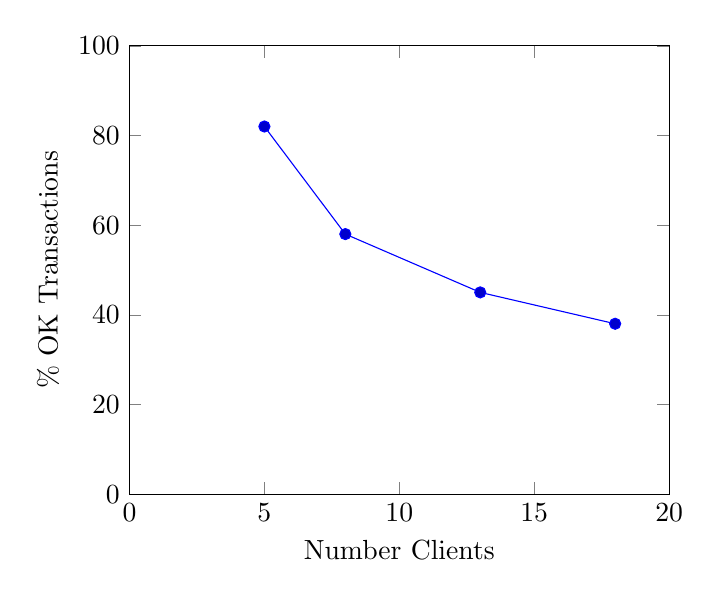
\begin{tikzpicture}
      \begin{axis}
        [
        xlabel={Number Clients},
        ylabel={\% OK Transactions},
        xmin=0, xmax=20,
        ymin=0, ymax=100,
        scaled x ticks = true,
        scaled y ticks = true,
        legend style={nodes=right},
        ]
        \addplot coordinates {
          (5, 82)
          (8, 58)
          (13, 45)
          (18, 38)
       };
      \end{axis}
    \end{tikzpicture}
    \captionof{figure}{Relation between number of clients and Ok Transactions}
    \label{fig:rel_cli_tx}
  \end{minipage}

  \item $(ii)$ Different number of entries

  \begin{table}[h!]
  \begin{tabular}{ |c|c|c|c| }
    \hline
    \multicolumn{4}{|c|}{Concurrent Clients - Duration 3s} \\
    \hline
    Experiment & Total Transactions & OK Transactions & \% Transactions\\
    \hline
    \multirow{4}{3cm}{3 CLIENTS \\ 5 ENTRIES \\ 1 RDxTR \\ 1 WRxTR}
    & 83714 & 79750 &  95.26483025539336 \%\\
    & 83462 & 79407 &  95.14150152165057 \%\\
    & 83683 & 79722 &  95.26666109006608 \%\\
    & & &\\
    \hline
    \multirow{4}{3cm}{3 CLIENTS \\ 10 ENTRIES \\ 1 RDxTR \\ 1 WRxTR}
    & 86061 & 83926 &  97.51920149661287 \%\\
    & 86258 & 84141 &  97.54573488835818 \%\\
    & 86285 & 84142 &  97.51637016862722 \%\\
    & & &\\
    \hline

    \multirow{4}{3cm}{3 CLIENTS \\ 15 ENTRIES \\ 1 RDxTR \\ 1 WRxTR}
    & 85535 & 84107 &  98.3305079791898 \%\\
    & 85691 & 84365 &  98.45257961746275 \%\\
    & 85738 & 84447 &  98.49424992418764 \%\\
    & & &\\

    \hline

    \multirow{4}{3cm}{3 CLIENTS \\ 20 ENTRIES \\ 1 RDxTR \\ 1 WRxTR}
    & 86984 & 85927 &  98.78483399245839 \%\\
    & 86733 & 85650 &  98.75134032029331 \%\\
    & 86756 & 85695 &  98.7770298307898 \%\\
    & & &\\

    \hline
  \end{tabular}
  \captionof{figure}{Results of several executions changing the number of entries in the Timestamp ordering algorithm}
  \label{table:timey_change_entries}
  \end{table}


  \item $(iii)$ Different number of reads per transaction

  \begin{table}[h!]
  \begin{tabular}{ |c|c|c|c| }
    \hline
    \multicolumn{4}{|c|}{Concurrent Clients - Duration 3s} \\
    \hline
    Experiment & Total Transactions & OK Transactions & \% Transactions\\
    \hline
    \multirow{4}{3cm}{3 CLIENTS \\ 5 ENTRIES \\ 1 RDxTR \\ 1 WRxTR}
    & 84802 & 80827 &  95.31261055163793 \%\\
    & 84585 & 80552 &  95.23201513270675 \%\\
    & 84694 & 80737 &  95.32788627293552 \%\\
    & & &\\
    \hline
    \multirow{4}{3cm}{3 CLIENTS \\ 5 ENTRIES \\ 6 RDxTR \\ 1 WRxTR}
    & 32364 & 29636 &  91.57088122605364 \%\\
    & 32377 & 29713 &  91.77193686876487 \%\\
    & 32353 & 29532 &  91.28056130807035 \%\\
    & & &\\
    \hline

    \multirow{4}{3cm}{3 CLIENTS \\ 5 ENTRIES \\ 11 RDxTR \\ 1 WRxTR}
    & 19417 & 17853 &  91.9452026574651 \%\\
    & 19428 & 17825 &  91.7490220300597 \%\\
    & 19403 & 17777 &  91.61985260011339 \%\\
    & & &\\

    \hline

    \multirow{4}{3cm}{3 CLIENTS \\ 5 ENTRIES \\ 16 RDxTR \\ 1 WRxTR}


    & 13542 & 12612 &  93.13247673903412 \%\\
    & 13548 & 12568 &  92.76645999409507 \%\\
    & 13545 & 12571 &  92.80915466961979 \%\\
    & & &\\
    \hline
  \end{tabular}
  \captionof{figure}{Results of several executions changing the number of reads per transaction in the Timestamp ordering algorithm}
  \label{table:timey_change_reads}
  \end{table}



  \item $(iv)$ Different number of writes per transaction

  \begin{table}[h!]
  \begin{tabular}{ |c|c|c|c| }
    \hline
    \multicolumn{4}{|c|}{Concurrent Clients - Duration 3s} \\
    \hline
    Experiment & Total Transactions & OK Transactions & \% Transactions\\
    \hline
    \multirow{4}{3cm}{3 CLIENTS \\ 5 ENTRIES \\ 1 RDxTR \\ 1 WRxTR}

    & 95082 & 90444 &  95.12210513030857 \%\\
    & 95221 & 90584 &  95.13027588452127 \%\\
    & 95247 & 90525 &  95.0423635390091 \%\\
    & & &\\
    \hline
    \multirow{4}{3cm}{3 CLIENTS \\ 5 ENTRIES \\ 1 RDxTR \\ 6 WRxTR}

    & 37820 & 23976 &  63.39502908514014 \%\\
    & 37752 & 23918 &  63.35558381012927 \%\\
    & 37876 & 23942 &  63.21153236878234 \%\\
    & & &\\
    \hline

    \multirow{4}{3cm}{3 CLIENTS \\ 5 ENTRIES \\ 1 RDxTR \\ 11 WRxTR}

    & 26477 & 12763 &  48.204101673150284 \%\\
    & 26405 & 12943 &  49.017231584927096 \%\\
    & 26421 & 12898 &  48.81722871957912 \%\\
    & & &\\
    \hline

    \multirow{4}{3cm}{3 CLIENTS \\ 5 ENTRIES \\ 4 RDxTR \\ 16 WRxTR}
    & 20541 & 8945 &  43.54705223698944 \%\\
    & 20573 & 8844 &  42.98838283186701 \%\\
    & 20514 & 8830 &  43.04377498293848 \%\\
    & & &\\
    \hline
  \end{tabular}
  \captionof{figure}{Results of several executions changing the number of writes per transaction in the Timestamp ordering algorithm}
  \label{table:timey_writes}
  \end{table}



  \item $(v)$ Different ratio in the number of reads and writes per transaction

  \begin{table}[h!]
  \begin{tabular}{ |c|c|c|c| }
    \hline
    \multicolumn{4}{|c|}{Concurrent Clients - Duration 3s} \\
    \hline
    Experiment & Total Transactions & OK Transactions & \% Transactions\\
    \hline
    \multirow{4}{3cm}{3 CLIENTS \\ 5 ENTRIES \\ 1 RDxTR \\ 1 WRxTR}

    & 96620 & 91978 &  95.19561167460154 \%\\
    & 96765 & 92206 &  95.28858574897949 \%\\
    & 96807 & 92279 &  95.32265228754119 \%\\
    & & &\\
    \hline
    \multirow{4}{3cm}{3 CLIENTS \\ 5 ENTRIES \\ 0 RDxTR \\ 10 WRxTR}
    & 25409 & 25154 &  98.99641859183754 \%\\
    & 25392 & 25151 &  99.05088216761185 \%\\
    & 25403 & 25150 &  99.00405463921584 \%\\
    & & &\\
    \hline

    \multirow{4}{3cm}{3 CLIENTS \\ 5 ENTRIES \\ 2 RDxTR \\ 8 WRxTR}

    & 28972 & 13556 &  46.79000414193014 \%\\
    & 29005 & 13599 &  46.885019824168246 \%\\
    & 28960 & 13397 &  46.2603591160221 \%\\
    & & &\\
    \hline

    \multirow{4}{3cm}{3 CLIENTS \\ 5 ENTRIES \\ 4 RDxTR \\ 6 WRxTR}
    & 27129 & 14496 &  53.43359504589185 \%\\
    & 27150 & 14524 &  53.49539594843462 \%\\
    & 27177 & 14685 &  54.03466166243515 \%\\
    & & &\\
    \hline
    \multirow{4}{3cm}{3 CLIENTS \\ 5 ENTRIES \\ 5 RDxTR \\ 5 WRxTR}
    & 26892 & 16020 &  59.57161981258367 \%\\
    & 26925 & 15989 &  59.38347260909935 \%\\
    & 26906 & 15872 &  58.99055972645507 \%\\
    & & &\\
    \hline

    \multirow{4}{3cm}{3 CLIENTS \\ 5 ENTRIES \\ 6 RDxTR \\ 4 WRxTR}


    & 26953 & 17735 &  65.79972544800208 \%\\
    & 26918 & 17734 &  65.88156623820493 \%\\
    & 26962 & 17795 &  66.00029671389363 \%\\
    & & &\\
    \hline
    \multirow{4}{3cm}{3 CLIENTS \\ 5 ENTRIES \\ 8 RDxTR \\ 2 WRxTR}

    & 26784 & 22065 &  82.38127240143369 \%\\
    & 26737 & 22085 &  82.60089015222351 \%\\
    & 26715 & 21967 &  82.22721317611828 \%\\
    & & &\\
    \hline
    \multirow{4}{3cm}{3 CLIENTS \\ 5 ENTRIES \\ 10 RDxTR \\ 0 WRxTR}

    & 29451 & 29451 &  100.0 \%\\
    & 29483 & 29483 &  100.0 \%\\
    & 29425 & 29425 &  100.0 \%\\
    & & &\\
    \hline

  \end{tabular}
  \captionof{figure}{Results of several executions changing the ratio if reads and writes per transaction in the Timestamp ordering algorithm}
  \label{table:timey_change_ratio}
  \end{table}

\end{itemize}
\end{document}
